\documentclass{article}
\usepackage[utf8]{inputenc}
\usepackage{lmodern}
\usepackage{amsmath}
\usepackage{parskip}
\usepackage[hyphens]{url}
\usepackage{graphicx}
\graphicspath{{./}}
\setlength{\skip\footins}{1cm}
\newcommand{\code}[1]{\colorbox{gray}{\texttt{#1}}}
\title{Hal\_3900 Proposal}
\begin{document}
\begin{LARGE}
\begin{center}
\vspace*{15mm}

COMP3900

Hal\_3900 Proposal

\rule[4.5pt]{0.61\textwidth}{0.3pt}

\begin{align*}
  \text{Ellen Oates}  \quad &\text{z5098896 \enspace Developer} \\
  \text{Hayden Le}    \quad &\text{z5098972 \enspace Developer} \\
  \text{Yi Wang}      \quad &\text{z5124282 \enspace Developer} \\
  \text{Zain Afzal}   \quad &\text{z5059449 \enspace Scrum Master}
\end{align*}

\rule[4.5pt]{0.61\textwidth}{0.3pt}

08/03/2019

\end{center}
\end{LARGE}

\vfill
\small{e.l.oates@unsw.edu.au}\\
\small{hayden.le@unsw.edu.au}\\
\small{z.afzal@unsw.edu.au}\\
\small{yi.wang7@student.unsw.edu.au}

\newpage

%-------------------------------------------------------------------------------------------------%

\tableofcontents 
\newpage
 
\section{Background}

\subsection{The Problem}
Online learning is changing the way students access and engage with higher education. Courses with online delivery increase the flexibility and accessibility of education by providing students with a platform to learn course content in their own time, at their own pace. Increasingly courses which are taught face to face include some online content delivery, including course materials, quizzes, online lecture recordings, and forums to ask questions and discuss the course content outside of class. Because online learning is so prevalent in higher education, it is crucial for universities to ensure students are satisfied with their learning experience. 

There is a delay between when students ask a question and when they get a response, and this can vary from hours to days. Answering individual student questions via email or on forums requires a significant amount of time for tutors, course administrators and lecturers. Often the same questions will be asked many times by different students, making it inefficient to have course staff respond to each one individually.

Some key factors that contribute to student satisfaction in the online learning space are:
\begin{itemize}
  \item Students' preferences for actively participating in learning, rather than through passive learning styles.
  \item Students' expectations on instructors to facilitate their learning by organising the course resources\footnote{\url{https://www.researchgate.net/publication/282699144_Student_Satisfaction_with_Online_Learning_Is_it_a_Psychological_Contract}}
  \item The amount of interaction students have with each other, and the availability of their instructors.\footnote{'Key Factors for Determining Student Satisfaction in Online Courses': \url{https://www.learntechlib.org/primary/p/2226/article_2226.pdf}}
  \item The availability of strong administrative support when using online learning tools or when confused about assessments and learning expectations.
  \item Course staff who are concerned with the quality of their course delivery, and want to know what their students need the most help with
  \item The availability of individual support and extended materials
\end{itemize}

Making these factors available to students becomes more challenging as classes grow in size. Course staff are thus in need of a more effective way to support with their students. 

\subsection{The Existing Solution}

Currently at UNSW, learning support is provided to students through email, forums and help sessions. This is very man-hour intensive, requiring many tutors to be on hand to answer questions which, of themselves, are quite repetitive. In addition, as these courses become larger with increasing enrollment sizes, it becomes more difficult to be able to give students individual attention.

Another side effect of growing cohort sizes is the fact that many tutors and lecturers are forced to spend most of their time answering admin related questions, which is time that could be spent improving the course. The current solution has been to hire more staff and offload the majority of questions to forums, however these are full of repeated questions and require many tutors to moderate them.

This growth is becoming unsustainable, and with the rise of online education platforms, many students are eager to interact with course material in a more meaningful way. Waiting for a tutor to respond often creates a disconnnect between the initial question and the answer, which limits the effectiveness of the response. This is provided that the tutor finds time to respond at all.

Chat bots have been deployed in some areas of secondary education, which interact with students in meaningful ways outside of class hours\footnote{\url{https://botsify.com/education-chatbot}}, and some have even been created to answer university-level questions\footnote{\url{https://www.canberra.edu.au/about-uc/media/newsroom/2018/february/students-make-new-friend-in-lucy-the-chatbot}}. However these tools can not be easily adopted by all university courses, or their administration and assessments.

\subsection{Our Solution}

The goal is to create a chat bot companion for students to enhance their learning experience. The chat bot will provide students with support by responding to their questions about course administration and the content they are learning in real time. In addition the bot will also monitor students' understanding of the course content with follow up questions. This is expected to increase both the amount and the quality of student interaction within the course. The bot provides students with more frequent and timely interactions. This helps by diverting more complex questions to tutors and lecturers, who in turn will have more time to respond to such questions in depth. 

The chat bot will provide administrative support by keeping students informed of their grades and upcoming due dates. This is expected to increase learning outcomes by boosting students' motivation to study. In addition, it will also enhance course delivery by keeping staff informed of their students' learning needs and frequently asked questions. It will reduce the load on course staff by answering many of the questions that students have and allowing them to focus on the overall delivery of the course. 

\subsection{Technical Details}

The technical stack of the chat bot will comprise several layers.

\begin{itemize}
  \item A frontend will be built in \texttt{Vue.js}
  \item A backend will be built in \texttt{Node.js}, providing \texttt{Websockets} to facilitate interactions with the frontend.
  \item \texttt{Dialogflow} will be used to parse user input and provide the natural language processing aspect of this project.
  \item \texttt{Actions} will be passed to the knowledge base of the bot, which will be built on top of \texttt{TensorFlow}, and will use machine learning to classify data and form connections between an input query and the relevant data points.
  \item Data will be stored on \texttt{Amazon S3} buckets.
\end{itemize}

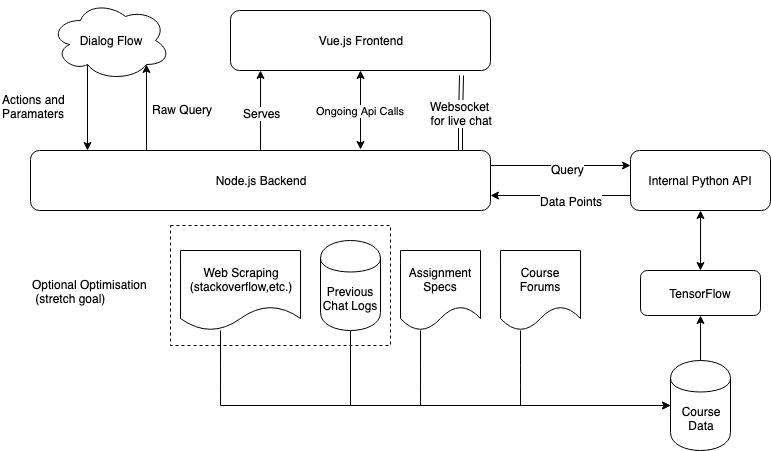
\includegraphics[width=\textwidth]{architecture_diagram.png}

The scope of this project is to have a bot which will answer a majority of basic administration questions, such as "when is assignment 1 due?". It will also respond to direct questions with a simple data point response, such as "how do you print with no new line in python" with a 50\% success rate. In addition the bot may have the ability to quiz students using a lecturer defined set of questions.


\section{Epics}

\subsection{Answers administrative questions about course}

The chatbot will be a course companion to clarify course administration details. It will answer questions regarding the following topics:
\begin{itemize}
  \item \textbf{Assignment management:} The requirements of assignments, relevant dates (release date, deadlines), weighting, and materials provided by the lecturer.
  \item \textbf{General information:} Locations of lectures, timetabling information, contact details of course staff, notices, teaching strategies, assumed knowledge and student learning outcomes.
  \item \textbf{Course Resources:} A list of textbooks, lecture recordings, relevant videos and external documents. 
\end{itemize}

This epic will be limited to questions that can be answered by referring to the the course homepage. Questions such as those regarding course content are beyond the scope of this epic.

This epic has an estimated difficulty of 7/10, because the core functionality does not rely on machione learning but the amount of data processing is significant. As such this epic has been assigned a time estimate of 4 units. 

\subsection{Answers questions about course content}
These questions make up a significant proportion of questions directed to tutors. Implementing this feature in the chat bot helps address the problem of tutors being expected to handle a large number of reptitive student questions. It will achieve this by:
\begin{itemize}
  \item Giving immediate answers to students, eliminating the need to wait for tutors' responses.
  \item Reducing workload of tutors, who are typically only paid for one hour of associated work.
  \item Answering questions beyond the scope of tutors' knowledge.
  \item Discouraging plagiarism by providing an officially endorsed information bank.
  \item Offering an outlet for shy students to ask questions in private.
\end{itemize}

The bot's knowledge base can be built from a number of sources. Apart from manual input, this can also include information scraped from appropriate sources such as course syllabus, lecture slides and past assignment submissions.

Information not directly related to the course content should be considered out of scope. However as there is no clear divide between what constitutes course content and what doesn't, there will be some degree of leniency as to what is included.

As one of the primary features, it has an estimated difficulty of 8/10 with a time estimate of 6 time units. That said, the actual implementation is not unlike that of epic 1, so there is potential for this epic to be leverage features implemented in  epic 1, as the functionality may be shared.

\subsection{Meaningfully quizzes and interacts with students}
The chat bot will be continuously trained and personalised to fit students' needs, as well as provide quizzes. Students can conveniently examine themselves to help determine areas for improvement. The chat bot's answers will increase in accuracy as it learns.

The epic comprises two fields:
\begin{itemize}
  \item \textbf{Statistics:} The chat bot will collate questions which the student has asked, to analyse students' strengths and weaknesses. In this way, future quizzes can be tailored to target points of confusion. These quizzes will be provided on demand. In addition, a summary of these statistics will also be provided to students, which will aid their personal study.
  \item \textbf{Personalisation:} The chat bot will interact with the students' and train itself according to the feedback it receives. This process will help students personalise the chatbots. Therefore, the chat bot can provide progressively more helpful answers.
\end{itemize}

The scope of this epic is limited to providing this personalisation for only one profile, and all conversations that occur will contribute towards developing this one profile. Moreover, the quiz questions will come from a pre-existing database. Further questions will not be included. This epic has an estimated difficulty score of 6/10, and a time stimate of 3.5 units.

\subsection{Informs course admin/staff about cohort}

This feature will allow the chat bot to maintain information about the questions users are asking, as well their performance in quizzes. This will be accessible from the admin web interface, available to course staff.

The main metrics that should be captured for a requested time frame are:
\begin{itemize}
  \item A list of the most common questions asked, and their relative frequency.
  \item A list of questions which the bot was unable to answer.
  \item A list of the questions or triggers for which the bot had a low satisfaction rating.
  \item A breakdown of every topic covered, and its retention rate among users, derived from interactive quizzing.
  \item General statistics on the bot's usage rate, uptime and the average computation time taken for a response.
\end{itemize}

The web interface will provide the ability to:
\begin{itemize}
  \item View interactive, sortable, tablular data for tracked metrics.
  \item View certain data, such as usage statistics and computation time as graphs.
  \item Export the metrics as \texttt{csv} or \texttt{json}.
  \item Register admin staff to be notified by email when certain conditions are met, for example, the bot is unable to answer over 50\% of student questions.
\end{itemize}

Any more additional advanced interaction with the data other than simple tabulation and graphing will be considered out of scope. Other forms of data visualisation should be deferred to specialist tools.

This epic aims to inform users of the bot's performance, and will not provide features to adjust the parameters of the bot. This is included in the second epic. 

As this is a difficult set of features to implement, its estimated difficulty is 7/10 with a time estimate of 4 time units.

\subsection{Learns to service new courses with a minimal setup process}

This feature will allow a course administrator to set up the chat bot to service the students in a given course with minimal configuration. The course administrator will be able to work through a short setup process to provide the chat bot with access to course materials and start giving students support for that course. 

The information provided by course administrators during setup will be:
\begin{itemize}
  \item Access to all course materials available to students.
  \item Course timetable and handbook information.
\end{itemize}

Following this setup process, the chat bot program will start ingesting the data, and no further setup will be required.

This epic has an estimated difficulty of 3/10, as it will combine significantly with the main implementation of the bot in epics 1 and 2. This epic has a time estimate of 3 units as a result. 


\section{Epic Selection}

Of the proposed epics, the following epics will be delivered in the final release:
\begin{itemize}
  \item Answers administrative questions about course.
  \item Answers questions about course content.
  \item Learns to service new courses with a minimal setup process.
\end{itemize}

Considering the goals of this project, these epics clearly outline the core functionality that should be achieved to deliver a minimum viable product. The main goal is to have a chat bot that students can direct questions to, and the epics were chosen accordingly.

The first two epics that were chosen directly correlate with the intended final outcome. Although the third epic is not directly related to this cause, it is an important feature required to perform the initial configuration of the chat bot, which is required to allow it to function normally.

The remaining epics are:
\begin{itemize}
  \item Meaningfully quizzes and interacts with students.
  \item Informs course admin/staff about cohort.
\end{itemize}

These epics go hand in hand to an extent, and while the features they provide are definitely useful, they are not essential to the basic functionality and upkeep of the chat bot. As such, they will be considered stretch goals which will be implemented if the scope of the project allows.


\section{Summary}

This project aims to deliver a chat bot that students can use as an assistant while taking certain courses. It will be implemented as a web application to provide an easy-to-use interface and developer-friendly code base to allow for extensibility. This is envisioned to address the problems that have been outlined in section 1.1 to a high degree, improve the learning experience for many students and extend staff teaching capabilities.

\end{document}
